%% abtex2-modelo-trabalho-academico.tex, v-1.9.6 laurocesar
%% Copyright 2012-2016 by abnTeX2 group at http://www.abntex.net.br/ 
%%
%% Modificado por Marcus Nunes para se adequar
%% às exigências do Departamento de Estatística
%% da Universidade Federal do Rio Grande do Norte
%% 
%% http://marcusnunes.me
%%
%% This work may be distributed and/or modified under the
%% conditions of the LaTeX Project Public License, either version 1.3
%% of this license or (at your option) any later version.
%% The latest version of this license is in
%%   http://www.latex-project.org/lppl.txt
%% and version 1.3 or later is part of all distributions of LaTeX
%% version 2005/12/01 or later.
%%
%% This work has the LPPL maintenance status `maintained'.
%% 
%% The Current Maintainer of this work is the abnTeX2 team, led
%% by Lauro César Araujo. Further information are available on 
%% http://www.abntex.net.br/
%%
%% This work consists of the files abntex2-modelo-trabalho-academico.tex,
%% abntex2-modelo-include-comandos and abntex2-modelo-references.bib
%%

% ------------------------------------------------------------------------
% ------------------------------------------------------------------------
% abnTeX2: Modelo de Trabalho Academico (tese de doutorado, dissertacao de
% mestrado e trabalhos monograficos em geral) em conformidade com 
% ABNT NBR 14724:2011: Informacao e documentacao - Trabalhos academicos -
% Apresentacao
% ------------------------------------------------------------------------
% ------------------------------------------------------------------------

\documentclass[
	% -- opções da classe memoir --
	12pt,				% tamanho da fonte
	openright,			% capítulos começam em pág ímpar (insere página vazia caso preciso)
	oneside,			% para impressão em recto e verso. Oposto a oneside
	a4paper,			% tamanho do papel. 
	% -- opções da classe abntex2 --
	%chapter=TITLE,		% títulos de capítulos convertidos em letras maiúsculas
	%section=TITLE,		% títulos de seções convertidos em letras maiúsculas
	%subsection=TITLE,	% títulos de subseções convertidos em letras maiúsculas
	%subsubsection=TITLE,% títulos de subsubseções convertidos em letras maiúsculas
	% -- opções do pacote babel --
	english,			% idioma adicional para hifenização
	french,				% idioma adicional para hifenização
	spanish,			% idioma adicional para hifenização
	brazil				% o último idioma é o principal do documento
	]{abntex2}

% ---
% Pacotes básicos 
% ---
\usepackage{multirow,lscape,array}
\usepackage{amsmath,amsthm,amssymb}
\usepackage{lmodern}			% Usa a fonte Latin Modern			
\usepackage[T1]{fontenc}		% Selecao de codigos de fonte.
\usepackage[utf8]{inputenc}		% Codificacao do documento (conversão automática dos acentos)
\usepackage{lastpage}			% Usado pela Ficha catalográfica
\usepackage{indentfirst}		% Indenta o primeiro parágrafo de cada seção.
\usepackage{color}				% Controle das cores
\usepackage{graphicx}			% Inclusão de gráficos
\usepackage{graphics}			% Inclusão de gráficos
\usepackage{amssymb}            % Inclusão de símbolos
\usepackage{microtype} 			% para melhorias de justificação
\usepackage{icomma}
\usepackage[final]{pdfpages}

% ---
		
% ---
% Pacotes adicionais, usados apenas no âmbito do Modelo Canônico do abnteX2
% ---
\usepackage{lipsum}				% para geração de dummy text
% ---

% ---
% Pacotes de citações
% ---
%\usepackage[brazilian,hyperpageref]{backref}	 % Paginas com as citações na bibl
\usepackage[alf]{abntex2cite}	% Citações padrão ABNT

% --- 
% CONFIGURAÇÕES DE PACOTES
% --- 

% ---
% Configurações do pacote backref
% Usado sem a opção hyperpageref de backref
%\renewcommand{\backrefpagesname}{Citado na(s) página(s):~}
% Texto padrão antes do número das páginas
%\renewcommand{\backref}{}
% Define os textos da citação
%\renewcommand*{\backrefalt}[4]{
%	\ifcase #1 %
%		Nenhuma citação no texto.%
%	\or
%		Citado na página #2.%
%%		Citado #1 vezes nas páginas #2.%
	%\fi}%
% ---

% ---
% Informações de dados para CAPA e FOLHA DE ROSTO
% ---
\titulo{Título da Monografia}
\autor{Nome do Discente}
\local{Natal - RN}
\data{7 de dezembro de 2017}
\orientador{Prof. Dr. Marcus Alexandre Nunes}
%\coorientador{Equipe \abnTeX}
\instituicao{%
  Universidade Federal do Rio Grande do Norte
  \par 
  Centro de Ciências Exatas e da Terra
  \par
  Departamento de Estatística
  \par
  }
  %Programa de Pós-Graduação}
\tipotrabalho{Monografia (Graduação)}
% O preambulo deve conter o tipo do trabalho, o objetivo, 
% o nome da instituição e a área de concentração 
\preambulo{Monografia de Graduação apresentada ao Departamento de Estatística do Centro de Ciências Exatas e da Terra da Universidade Federal do Rio Grande do Norte como requisito parcial para a obtenção do grau de Bacharel em Estatística.}
% ---


% ---
% Configurações de aparência do PDF final

% alterando o aspecto da cor azul
\definecolor{blue}{RGB}{41,5,195}

% informações do PDF
\makeatletter
\hypersetup{
     	%pagebackref=true,
		pdftitle={\@title}, 
		pdfauthor={\@author},
    	pdfsubject={\imprimirpreambulo},
	    pdfcreator={LaTeX with abnTeX2},
		pdfkeywords={Má especificação}{Estatísticas Robustas}{Família de Posição e Escala}{Modelos de Regressão}{Estatística Gradiente}, 
		bookmarksdepth=4
}
\makeatother
% --- 

% --- 
% Espaçamentos entre linhas e parágrafos 
% --- 

% O tamanho do parágrafo é dado por:
\setlength{\parindent}{1.3cm}

% Controle do espaçamento entre um parágrafo e outro:
\setlength{\parskip}{0.2cm}  % tente também \onelineskip

\theoremstyle{plain}
\newtheorem{theorem}{Teorema}[section]
\newtheorem{axiom}{Axioma}[section]
\newtheorem{corollary}{Corolário}[section]
\newtheorem{lemma}{Lema}[section]
\newtheorem{proposition}{Proposição}[section]
%-----------------------------------------------------------
\theoremstyle{definition}
\newtheorem{definition}{Definição}[section]
\newtheorem{example}{Exemplo}[section]
%-----------------------------------------------------------
\theoremstyle{remark}
\newtheorem{remark}{Observação}[section]

% ---
% compila o indice
% ---
\makeindex
% ---
\newcommand{\R}{\mathbb{R}}
\newcommand{\N}{\mathbb{N}}
\newcommand{\Z}{\mathbb{Z}}
\newcommand{\Q}{\mathbb{Q}}

\newcommand{\marcus}[2]{\textcolor{red}{#1}\footnote{Marcus: #2}\xspace}

% ----
% Início do documento
% ----
\begin{document}

% Seleciona o idioma do documento (conforme pacotes do babel)
%\selectlanguage{english}
\selectlanguage{brazil}

% Retira espaço extra obsoleto entre as frases.
\frenchspacing 


% ----------------------------------------------------------
% ELEMENTOS PRÉ-TEXTUAIS
% ----------------------------------------------------------
% \pretextual

% ---
% Capa
% ---
\imprimircapa
% ---

% ---
% Folha de rosto
% (o * indica que haverá a ficha bibliográfica)
% ---
\imprimirfolhaderosto*

% ---

% ---
% Inserir a ficha bibliografica
% ---

% Isto é um exemplo de Ficha Catalográfica, ou ``Dados internacionais de
% catalogação-na-publicação''. Você pode utilizar este modelo como referência. 
% Porém, provavelmente a biblioteca da sua universidade lhe fornecerá um PDF
% com a ficha catalográfica definitiva após a defesa do trabalho. Quando estiver
% com o documento, salve-o como PDF no diretório do seu projeto e substitua todo
% o conteúdo de implementação deste arquivo pelo comando abaixo:
%
 \begin{fichacatalografica}
 	% editar a linha abaixo com a ficha catalografica
 	% fornecida pela biblioteca
    %\includepdf{FichaCatalografica.pdf}
 \end{fichacatalografica}



% ---
% Inserir folha de aprovação
% ---

% Isto é um exemplo de Folha de aprovação, elemento obrigatório da NBR
% 14724/2011 (seção 4.2.1.3). Você pode utilizar este modelo até a aprovação
% do trabalho. Após isso, substitua todo o conteúdo deste arquivo por uma
% imagem da página assinada pela banca com o comando abaixo:
%
%
% editar a linha abaixo com a folha de aprovacao
% fornecida pela biblioteca
%\includepdf{FolhadeRos.pdf}
\begin{folhadeaprovacao}

  \begin{center}
    {\ABNTEXchapterfont\large\imprimirautor}

    \vspace*{\fill}\vspace*{\fill}
    \begin{center}
      \ABNTEXchapterfont\bfseries\Large\imprimirtitulo
    \end{center}
    \vspace*{\fill}
    
    \hspace{.45\textwidth}
    \begin{minipage}{.5\textwidth}
        \imprimirpreambulo
    \end{minipage}%
    \vspace*{\fill}
   \end{center}
        
   Aprovado em \hphantom{XXX} de \hphantom{XXXXXXXXXXX} de \hphantom{XXXXXX}.

   \assinatura{\textbf{\imprimirorientador} \\ Orientador} 
   \assinatura{\textbf{Profª. Drª. Fulana} \\ Examinadora}
   \assinatura{\textbf{Prof. Dr. Beltrano} \\ Examinador}
   %\assinatura{\textbf{Professor} \\ Convidado 3}
   %\assinatura{\textbf{Professor} \\ Convidado 4}
      
   \begin{center}
    \vspace*{0.5cm}
    {\large\imprimirlocal}
    \par
    {\large\imprimirdata}
    \vspace*{1cm}
  \end{center}
  
\end{folhadeaprovacao}
% ---

% ---
% Dedicatória
% ---
\begin{dedicatoria}
   \vspace*{\fill}
   \flushright
   \noindent
   \textit{Alguém importante.} \vspace*{3cm}
\end{dedicatoria}
% ---

% ---
% Agradecimentos
% ---
\begin{agradecimentos}

A todo mundo que é importante.

\end{agradecimentos}
% ---

% ---
% Epígrafe
% ---
\begin{epigrafe}
    \vspace*{\fill}
	\begin{flushright}
		\textit{``Uma frase legal.'' \\
		Autor da frase legal} \vspace*{3cm}
	\end{flushright}
\end{epigrafe}
% ---

% ---
% RESUMOS
% ---

% resumo em português
\setlength{\absparsep}{18pt} % ajusta o espaçamento dos parágrafos do resumo
\begin{resumo}
Resumo da monografia.

 \textbf{Palavras-chave}: Palavras. Chave. Separadas por Ponto.
\end{resumo}

% resumo em inglês
\begin{resumo}[Abstract]
 \begin{otherlanguage*}{english}
Abstract in english.

   \vspace{\onelineskip}
 
   \noindent 
   \textbf{Keywords}: Keywords. Dot separated.
 \end{otherlanguage*}
\end{resumo}
% ---


% ---
% inserir lista de ilustrações
% ---
\pdfbookmark[0]{\listfigurename}{lof}
\listoffigures*
\cleardoublepage
% ---


% ---
% inserir lista de tabelas
% ---% ---
\pdfbookmark[0]{\listtablename}{loc}
\listoftables
\cleardoublepage

% ---
% inserir lista de abreviaturas e siglas
% ---
% inserir lista de símbol
% ---
% inserir o sumario
% ---
\pdfbookmark[0]{\contentsname}{toc}
\tableofcontents* 
\cleardoublepage
% ---



% ----------------------------------------------------------
% ELEMENTOS TEXTUAIS
% ----------------------------------------------------------
\textual


\renewcommand{\thetable}{\thechapter.\arabic{table}}
\setcounter{table}{0}
\renewcommand{\thefigure}{\thechapter.\arabic{figure}}
\setcounter{figure}{0}
\renewcommand{\theequation}{\thechapter.\arabic{equation}}
\setcounter{equation}{0}

\chapter{Introdução}\label{introducao}

Utilize este espaço para escrever a introdução da sua monografia. Ela deve ter as seguintes características:

\begin{itemize}

  \item Tema bem delimitado, apresentando qual a função do seu trabalho
  \item O texto deve ser breve
  \item Apresente o problema da pesquisa da sua monografia
  \item Descreva a relevância do tema escolhido e do trabalho realizado
  \item Apresente os objetivos geral (ideia central) e específicos (resultados a serem atingidos)
  \item De forma sucinta, comente sobre os instrumentos e métodos utilizados para desenvolver seu trabalho
  \item Escreva um parágrafo como este abaixo, com a estrutura dos capítulos

\end{itemize}

A revisão bibliográfica e nossa motivação é feita no Capítulo \ref{revisaobibliografica}. Descrevemos o modelo estudado neste trabalho no Capítulo \ref{modelagem}. O Capítulo \ref{resultados} trata dos resultados dos estudos realizados. A conclusão é feita no Capítulo \ref{consideracoesfinais}.

Os capítulos listados acima são apenas uma sugestão de organização da monografia. A quantidade de capítulos pode ser aumentada ou diminuída de acordo com a preferência do aluno e do orientador.



\renewcommand{\thetable}{\thechapter.\arabic{table}}
\setcounter{table}{0}
\renewcommand{\thefigure}{\thechapter.\arabic{figure}}
\setcounter{figure}{0}
\renewcommand{\theequation}{\thechapter.\arabic{equation}}
\setcounter{equation}{0}

\chapter{Revisão Bibliográfica}\label{revisaobibliografica}

Aqui listamos os artigos e livros importantes para este trabalho. É importante procurar referências na literatura, sejam em livros, artigos ou outros trabalhos de conclusão, que fundamentem o seu trabalho. As referências podem trazer informações, conceitos e metodologias a serem utilizadas.

Com as fontes coletadas, analise-as para determinar como elas se relacionam com o seu trabalho. Estas fontes podem ser uma base teórica para o trabalho ou podem ser uma aplicação similar à sua proposta. Elas, inclusive, podem possuir deficiências para as quais o seu trabalho está buscando soluções.

Construa uma estrutura capaz de organizar os seus referenciais teóricos, de modo a ordená-los dentro do recorte do seu trabalho. Crie uma relação entre os trabalhos, relacionando-os entre si e entre os objetivos da monografia.

Em um trabalho sobre regressão utilizando dados de contagem, os livros \citeonline{Hilbe2011} e \citeonline{Nelder1989} são fundamentais para a base teórica dos modelos lineares generalizados que tratam de dados deste tipo. São livros com a parte teórica muito bem desenvolvida. 

Todos os referenciais teóricos devem estar dentro do arquivo \texttt{bibliografia}, no formato utilizado pelo BibTeX.  




\renewcommand{\thetable}{\thechapter.\arabic{table}}
\setcounter{table}{0}
\renewcommand{\thefigure}{\thechapter.\arabic{figure}}
\setcounter{figure}{0}
\renewcommand{\theequation}{\thechapter.\arabic{equation}}
\setcounter{equation}{0}

\input{03-Modelagem}

\renewcommand{\thetable}{\thechapter.\arabic{table}}
\setcounter{table}{0}
\renewcommand{\thefigure}{\thechapter.\arabic{figure}}
\setcounter{figure}{0}
\renewcommand{\theequation}{\thechapter.\arabic{equation}}
\setcounter{equation}{0}

\chapter{Resultados}\label{resultados}

Os resultados vem aqui.

\section{Simulação}\label{resultadosSimulacao}

É possível criar seções e subseções dentro do documento. Isso vai deixar o trabalho mais organizado.




\subsection{Simulação Particular}\label{resultadosSimulacao_sub}

Escreva neste local resultados particulares de alguma simulação realizada, caso isso seja necessário.



\section{Aplicação}\label{aplicacao}

Aplicação a dados reais do método descrito no Capítulo \ref{modelagem}. A Figura \ref{serietemporal} mostra os dados analisados neste trabalho. 


\begin{figure}[!h]
\centering
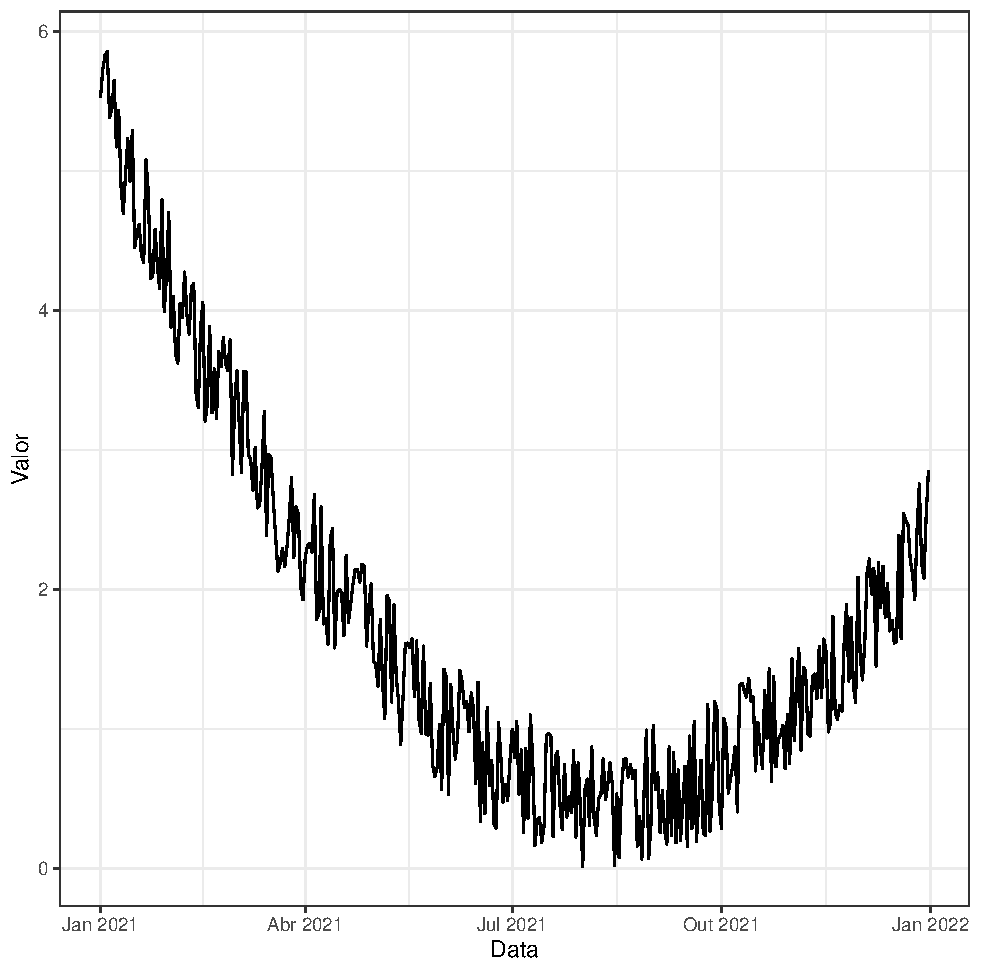
\includegraphics[width=0.8\textwidth]{figuras/serie_temporal.pdf}
\label{serietemporal}
\end{figure}


Devido a características do próprio LaTeX, as figuras podem acabar ficando em posições estranhas às vezes. Em geral, quanto mais texto for escrito, mais fácil é para o programa encontrar locais mais adequados para as figuras.


\marcus{Este comando é interessante. Ele está definido na linha 186 do arquivo 00-Monografia.tex.}{Com este comando, é possível o orientador fazer comentários mais efetivos na correção do texto do aluno, caso ambos estejam usando o Overleaf para trabalhar.}


\renewcommand{\thetable}{\thechapter.\arabic{table}}
\setcounter{table}{0}
\renewcommand{\thefigure}{\thechapter.\arabic{figure}}
\setcounter{figure}{0}
\renewcommand{\theequation}{\thechapter.\arabic{equation}}
\setcounter{equation}{0}

\chapter{Considerações Finais}\label{consideracoesfinais}

Utilize este espaço para retomar o tema do trabalho, destacando as suas contribuições acadêmicas. Dê uma pequena retomada na metodologia utilizada.

Avalie se a monografia cumpriu o que ela prometia na introdução. 

Feche o seu trabalho, apresentando os resultados obtidos de maneira resumida, utilizando apenas informações e resultados constantes na monografia. É algo pessoal, que deve refletir a sua opinião sobre o trabalho realizado.

Relembre a hipótese ou proposta do trabalho, avaliando se ela foi confirmada ou refutada. Explique o porquê da sua opinião.

\section{Propostas de Trabalhos Futuros}

Por fim, crie uma seção com propostas de futuros trabalhos. Proponha novas ideias para serem trabalhadas futuramente, apontando caminhos que possam ser trilhados pelo autor do trabalho ou por outras pessoas da área.


\bibliography{bibliografia}



\end{document}
